\documentclass[20pt, twoside]{extbook}
\usepackage{graphicx}
\usepackage{multicol}
\usepackage{marginnote}
\usepackage{etoolbox}
\usepackage{setspace}
\usepackage[font={small,it}]{caption}
\usepackage{titlesec}
\usepackage{subfig}
\usepackage{float}
\usepackage[latin.classical]{babel}

\captionsetup[figure]{labelfont={bf},labelformat={default},labelsep=none,name={},belowskip=-10pt}

\newcommand{\ki}[1]{%
    \begin{figure}[h!]
            %\centering
            %\setlength{\fboxsep}{0pt}
            \includegraphics{#1}
    \end{figure}}

\newcommand{\kimg}[2]{%
    \begin{figure}[h]
            \centering
            \setlength{\fboxsep}{0pt}
            \fbox{\includegraphics{#1}}
            \caption{#2}
    \end{figure}}

\newcommand{\mimg}[2]{%
    \marginpar{\begin{center}\includegraphics{#1}\\#2\end{center}}}

\titleformat{\chapter}
{\normalfont\bfseries}
{}{0em}{}
\titlespacing*{\chapter}{0pt}{-50pt}{20pt}

\titleformat{\section}
{\normalfont\bfseries}
{}{0em}{}
\titlespacing*{\section}{0pt}{5pt}{10pt}

\renewcommand{\thefigure}{}

\let\oldmarginpar\marginpar
\renewcommand\marginpar[1]{\oldmarginpar[\raggedleft\scriptsize #1]%
{\raggedright\scriptsize #1}}

\usepackage[top=1.5cm, bottom=2cm, outer=7cm, inner=2cm, heightrounded, marginparwidth=6.25cm, marginparsep=0.5cm]{geometry}
\marginparpush 1ex
\setlength{\columnsep}{1cm}
\newcommand{\rnc}[1]
    {\MakeUppercase{\romannumeral #1}}
\parskip 1.5ex
\pagestyle{plain}
\begin{document}

\mainmatter

\chapter{CAPITULUM PRIMUM}

\begin{figure}[p]
    \hspace*{-2.5cm}
    \makebox[\linewidth]{
        \setlength{\fboxsep}{0pt}
        \fbox{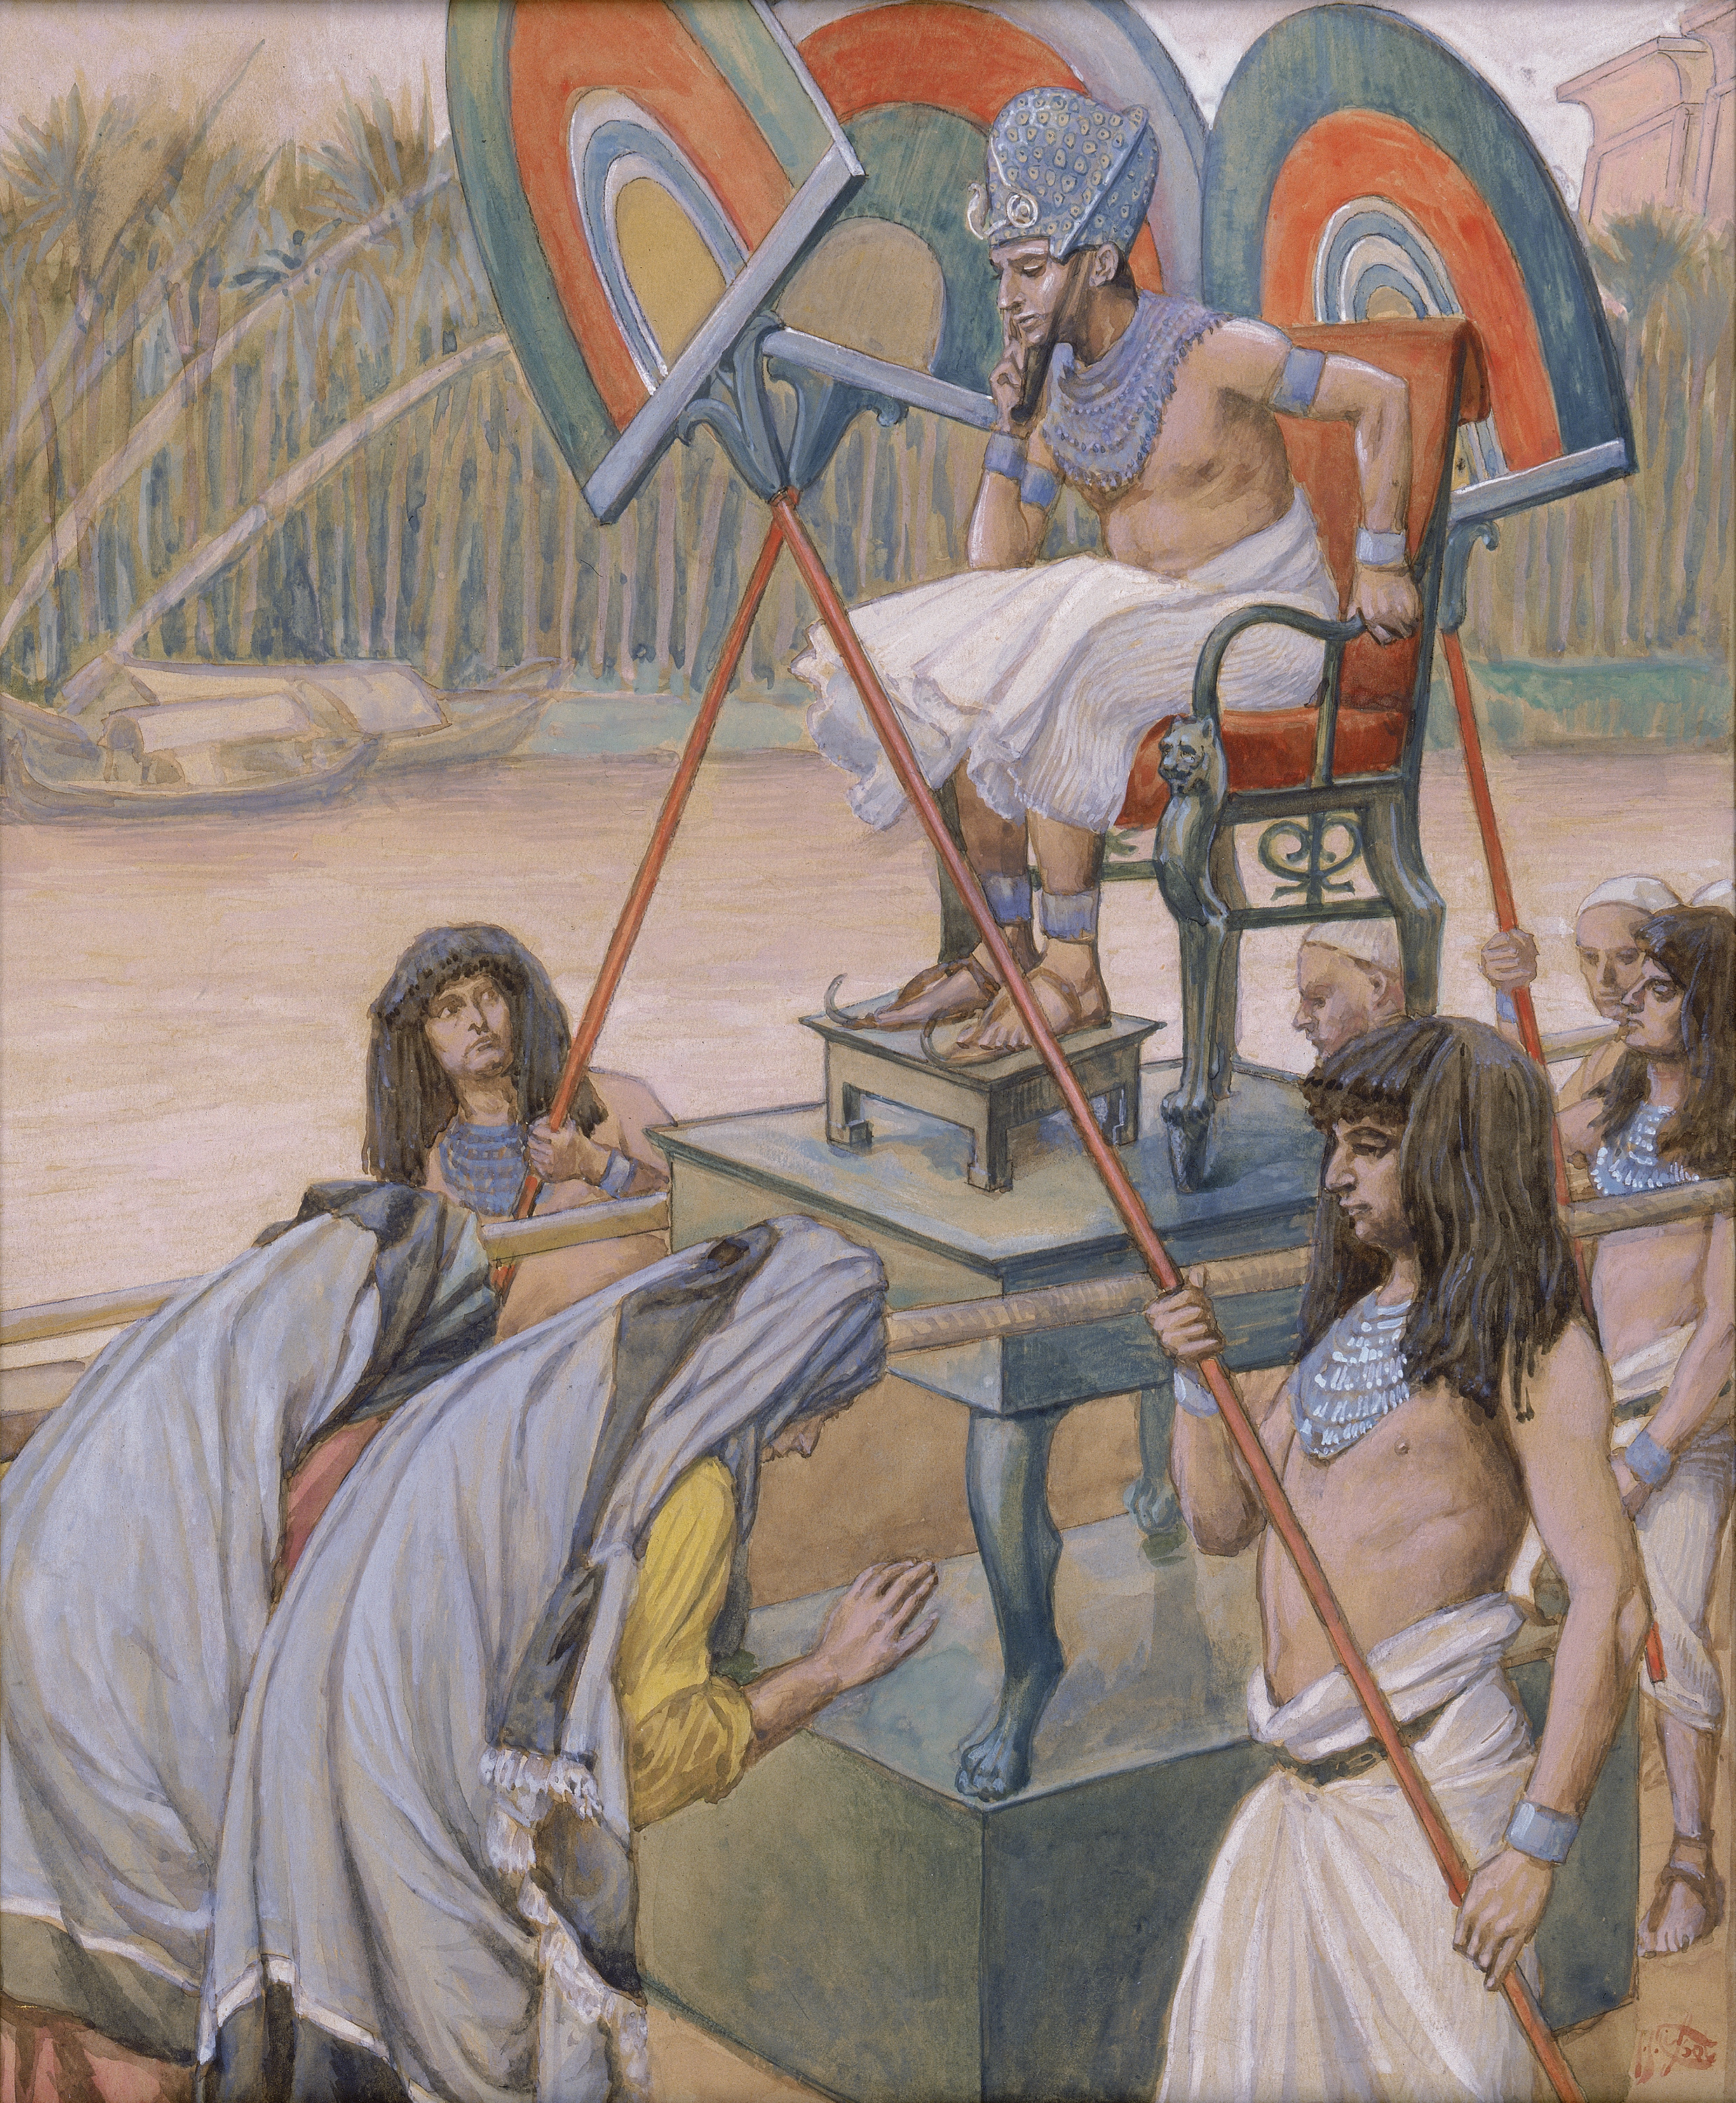
\includegraphics[width=1.3\linewidth]{midwives}}
    }
    \caption{\hspace*{-4.5cm}Obstetricēs et Rēx}
\end{figure}

\marginpar{quasi: velut}[In Aegyptō] fīliī Isrāēl crēvērunt, et quasi\marginpar{germināre: emmitere germina (ea quae ex plantīs veniunt: semen, fructus, cēt.)} germinantēs multiplicātī sunt:
ac rōborātī \marginpar{rōborāre: firmāre; virēs addere}nimis, implēvērunt terram.

Surrēxit intereā rēx novus super Ægyptum, quī ignōrābat Ioseph.
Et ait ad populum suum: ``Ecce, populus fīliōrum Isrāēl multus, et fortior nōbīs est.
\marginpar{ingruere: cum vi accedere}Venīte, sapienter opprimāmus eum, nē forte multiplicētur: et sī ingruerit contrā nōs bellum, addātur inimīcīs nostrīs, expugnātisque nōbīs ēgrediātur dē terrā.''\marginpar{\begin{center}
\includegraphics{tab}\\tabernaculum, -ī (n)\end{center}tabernaculum quoque significat aedificium sacrum, ad formam tabernaculī}

\marginpar{praeposuit eīs magistrōs operum: dedit magistrīs potestatem super opera fīliōrum Isrāēl}
Præposuit itaque eīs magistrōs operum, ut afflīgerent eōs oneribus: 
ædificaveruntquē urbēs tabernāculōrum Pharaōnī, Phithom et Ramessēs.
Quantōque opprimēbant eōs, tantō magis multiplicābantur, et crēscēbant: 
ōderantque fīliōs Isrāēl Ægyptiī, et afflīgēbant \marginpar{illūdere: deridēre}illūdentēs eīs,
atque ad amāritūdinem perdūcēbant vītam eōrum operibus dūrīs \marginpar{lutum, -ī(n): terra humida}lutī et lateris, omnīque famulātū, quō in terræ operibus premēbantur. 
Dīxit autem rēx Ægyptī \marginpar{obstetrix, -īcis(f): femina quae iuvat feminam gravidam parere} obstetrīcibus Hebræōrum, quārum ūna vocābātur Sephora, altera Phua, 
præcipiēns eīs: ``Quandō obstetrīcābitis Hebræās, et \marginpar{partus, -ūs (m): actus pariendi} partus tempus advēnerit: sī masculus fuerit, interficite eum: sī fēmina, \marginpar{reservāre: servāre, conservāre}reservātē.''

\marginpar{nōn fēcērunt iuxtā praeceptum regis: non parent praeceptō rēgis}\marginpar{mas, maris(m): homo (vel animal) masculinus}Timuērunt autem obstetrīcēs Deum, et nōn fēcērunt iuxtā præceptum rēgis Ægyptī, sed cōnservābant marēs. 
Quibus ad sē accersītis, rēx ait: ``Quidnam est hoc quod facere voluistis, ut puerōs servārētis?''

Quæ respondērunt: ``Nōn sunt Hebreæ sīcut Ægyptiæ mulierēs: ipsæ enim obstetrīcandī habent scientiam, et priusquam veniāmus ad eās, pariunt.''

\marginpar{cōnfortāre: fortem facere, consolārī}Bene ergō fēcit Deus obstetrīcibus: et crēvit populus, cōnfortātusque est nimis.
Et quia timuērunt obstetrīcēs Deum, ædificāvit eīs domōs.
Præcēpit ergō Pharaō omnī populō suō, dīcēns: ``Quidquid masculīnī sexūs nātum fuerit, in flūmen prōiicite: quidquid fēminīnī, reservātē.''

\section{Quaestiō Augustīnī}

{\it Dē obstetrīcum mendāciō, quō fefellērunt Pharaōnem, nē
occīderent masculōs Isrā-ēlītās quandō nāscēbantur, dīcentēs
nōn ita pārēre mulierēs Hebraēās sīcut pariēbant Aegyptiae:}

Quaerī solet utrum tālia mendācia approbāta sint
auctōritāte dīvīnā, quandōquidem scrīptum est Deum
bene fēcisse obstetrīcibus: sed utrum prō misericordiā
ignōscēbat mendāciō; an et ipsum mendācium dignum
praemiō iūdicābat, incertum est.

\marginpar{vīvificāre: vivum facere, vitam dare}Aliud enim faciēbant obstetrīcēs vīvificandō
īnfantēs parvulōs, aliud Pharaōnī mentiendō: nam
in illīs vīvificandīs opus misericordiae fuit; mendāciō
vērō illō prō sē ūtēbantur, nē nocēret illīs
Pharaō, quod potuit nōn ad laudem, sed ad veniam pertinēre.

\marginpar{id est, ut ita dīcam, haec fābula nōn dat licentiam mentiendī}Neque hinc auctōritātem ad mentiendum esse prōpositam
\marginpar{eōrum: sanctōrum}mihi vidētur eīs dē quibus dictum est: ``Et nōn est
inventum in ōre eōrum mendācium.''

Quōrumdam enim vīta longē
īnferior ā professiōne sānctōrum, sī habeat ista
mendāciōrum peccāta, prōvectū ipsō et indole feruntur,
\marginpar{{\bf nōrunt} = nōvērunt}praesertim sī beneficia dīvīna nōndum nōrunt exspectāre
coelestia, sed circā terrēna occupantur.

\marginpar{conversātiō, -ōnis (f): modus vīvendī}Quī autem ita vīvunt, ut eōrum conversātiō,
sīcut dīcit Apostolus,
in coelīs sit, nōn eōs exīstimō linguae suae modum,
\marginpar{non exīstimō eōs debēre formāre modum linguae suae exemplō illō obstetrīcum}
quantum ad vēritātem prōmendam attinet falsitātemque vītandam,
exemplō illō obstetrīcum dēbēre fōrmāre.

\marginpar{disserere: sermōnem īnstituere dē rē aliquā, dīcere, disputāre, tractāre}Sed dīligentius dē hāc quaestiōne disserendum est,
propter alia exempla quae in Scrīptūrīs reperiuntur.

\begin{figure}[bp]
    \hspace*{-2.5cm}
    \makebox[\linewidth]{
        \setlength{\fboxsep}{0pt}
        \fbox{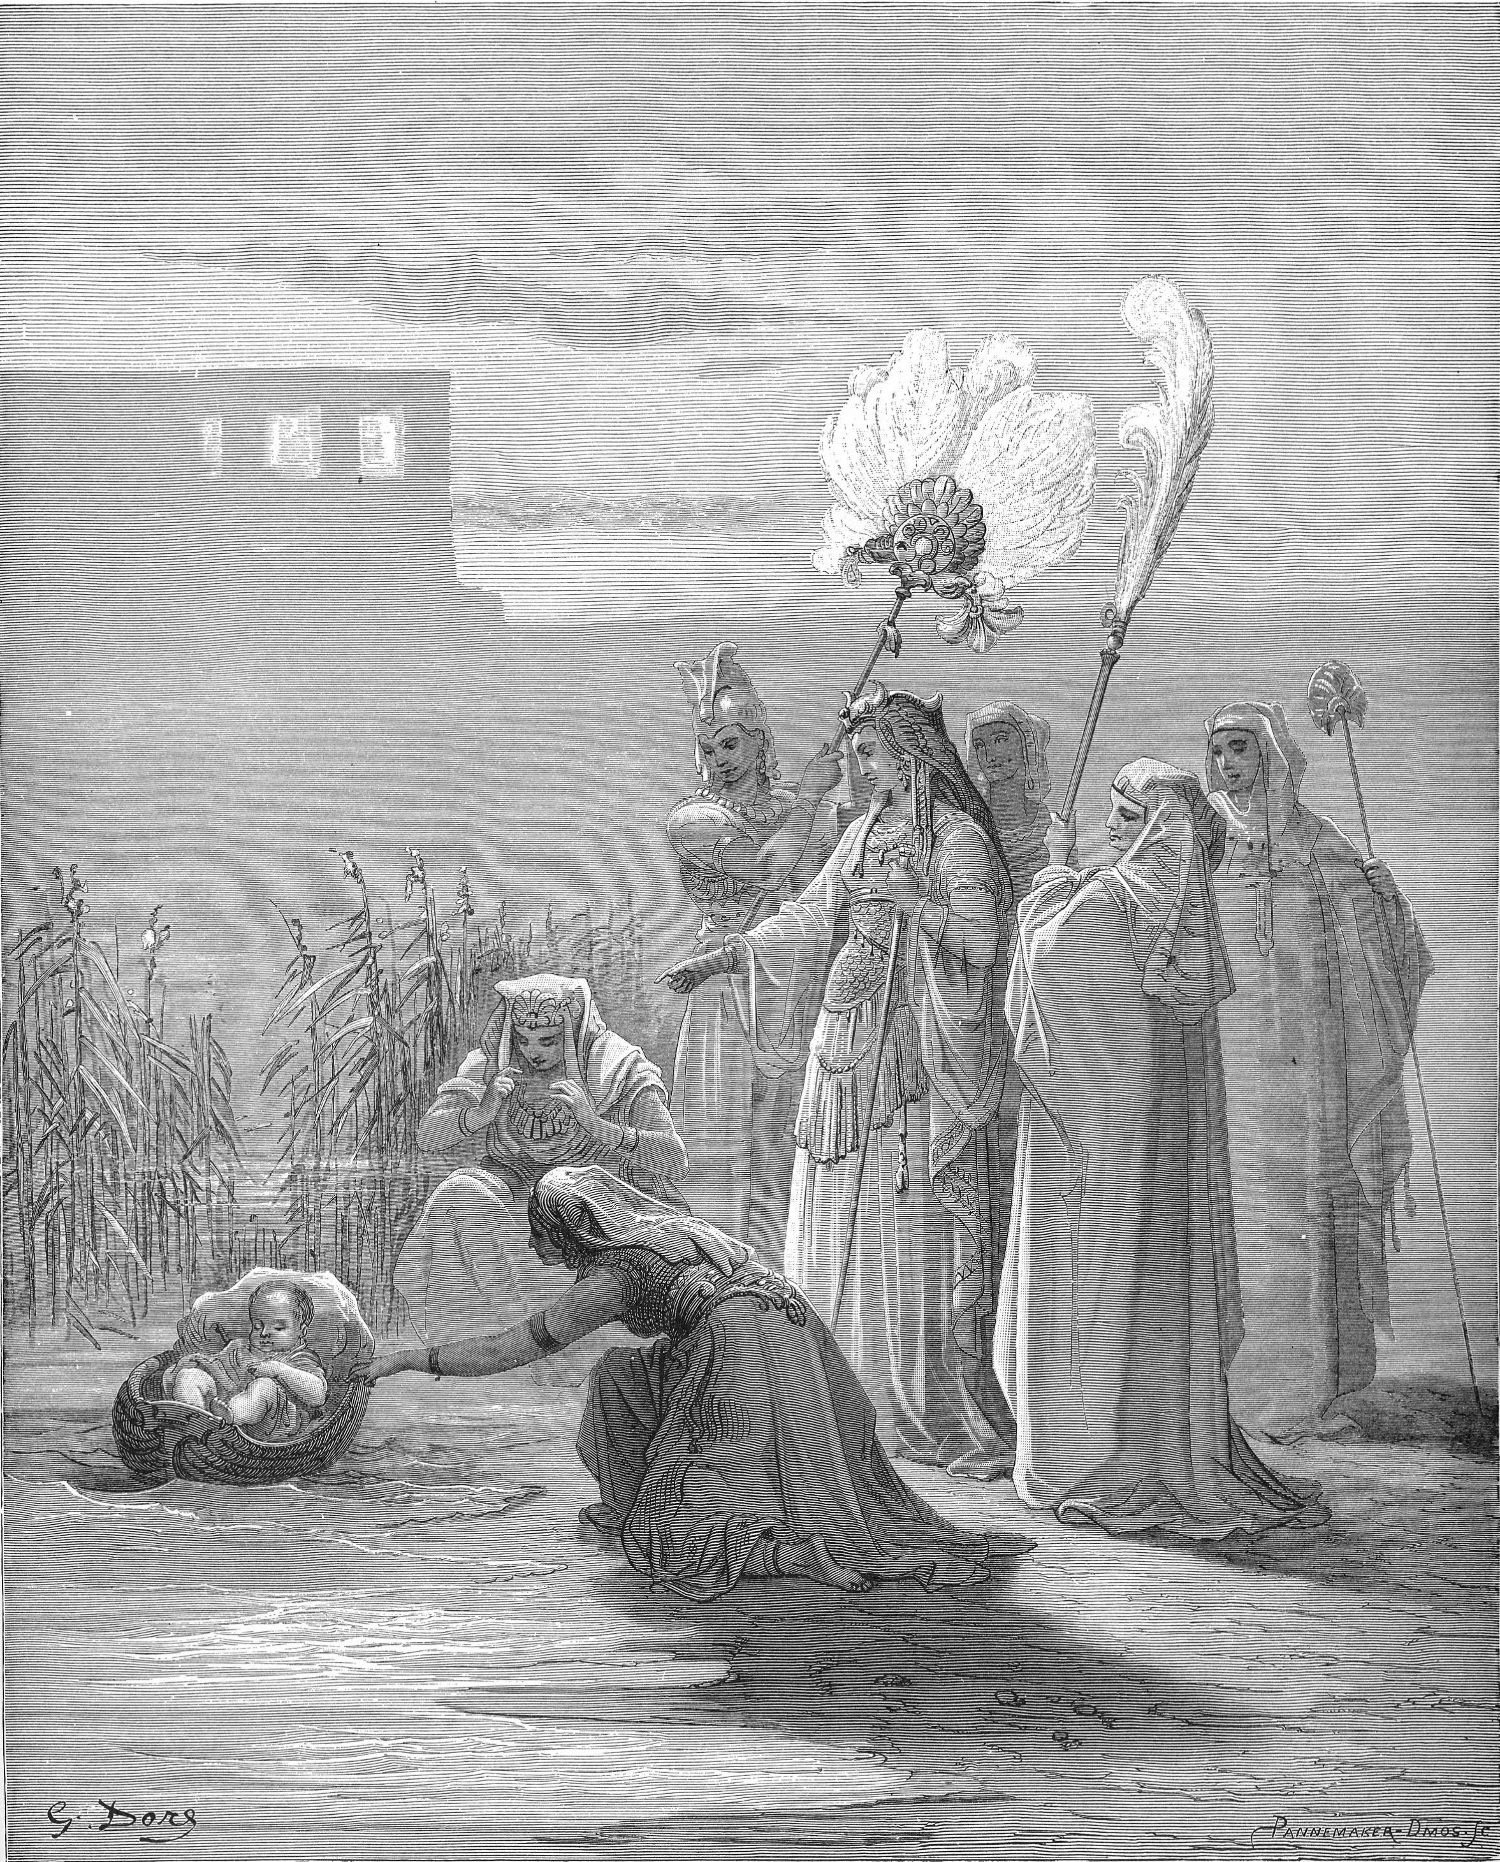
\includegraphics[width=1.3\linewidth]{babymoses.jpg}}
    }
    \caption{\hspace*{-4cm}Infans Moysēs}
\end{figure}

\chapter{CAPITULUM SECUNDUM}
\marginpar{stirps, stirpis(m/f): stricto sensu est truncus arboris, ergo etiam origo est generis in familiis}Ēgressus est post hæc vir dē domō Levī: et accēpit uxōrem stirpis suæ.
Quæ concēpit, et peperit fīlium : et vidēns eum ēlegantem, abscondit tribus mēnsibus.
\marginpar{scirpeus/a/um: ex scirpīs factus}
\marginpar{linere: rem aliquam liquidam aut mollem alteri superinducere}
\marginpar{bitūmen, -inis(n): limus pinguis et sulphureus ē terrā emergens pluribus locīs}
\marginpar{pix, picis (f): rēs ātra quae fit ex liquōre crassō arborum coctō}
\marginpar{cārex, cāricis (f):  herba acuta et durissima, sparto similis}
\marginpar{cārectum, -ī (n): locus caricibus plenus}

\begin{figure}[hp]
    \begin{minipage}[hbp]{0.5\linewidth}
        \centering
        
\includegraphics{fisc}
        \caption{fiscella, -ae(f)}
    \end{minipage}%
    \begin{minipage}[hbp]{0.5\linewidth}
        \centering
        
\includegraphics{brush}
        \caption{scirpus, -ī(m)}
    \end{minipage}
\end{figure}

Cumque iam cēlāre nōn posset, sūmpsit fiscellam scirpeam,
et līnīvit eam bitūmine ac pice:
posuitque intus īnfantulum, et exposuit eum in cārectō rīpæ flūminis,
stante procul sorōre eius, et cōnsīderante ēventum reī.
Ecce autem dēscendēbat fīlia Pharaōnis ut lavārētur in flūmine.\marginpar{crepīdo, -inis (f): litus maris vel ripa fluminis, quae saxis, aut lapideo margine plerumque sternebantur}\marginpar{alveus, -ī (m): fossa, per quam fluvius defluit} Et puellæ eius gradiēbantur per crepīdinem alveī.
\marginpar{papyrio, -ōnis (m): locus papyrīs consitus}
Quæ cum vīdisset fiscellam in papȳriōne,
mīsit ūnam ē famulābus suīs: et allātam aperiēns,
cernēnsque in eā parvulum vāgientem,
miserta eius, ait: ``Dē īnfantibus Hebræōrum est hīc.''

Cui soror puerī: ``Vīs,'' inquit, ``ut vādam, et vōcem tibi mulierem hebræam,
quæ nūtrīre possit īnfantulum?''

Respondit: ``Vāde.''

Perrēxit puella et vocāvit mātrem suam.
Ad quam locūta fīlia Pharaōnis: ``Accipe,'' ait, ``puerum istum, et nūtrī mihi: ego dabō tibi mercēdem tuam.''

Suscēpit mulier, et nūtrīvit puerum: adultumque trādidit fīliæ Pharaōnis. 
Quem illa adoptāvit in locum fīliī,
vocāvitque nōmen eius Moysēs, dīcēns: ``Quia dē aquā tulī eum.''

In diēbus illīs postquam crēverat Moysēs, ēgressus est ad frātrēs suōs:
\marginpar{percutere: pulsare, afficere, et quasi vulnerare dolore}vīditque afflīctiōnem eōrum, et virum ægyptium percutientem quemdam dē Hebræīs frātribus suīs.
Cumque circumspexisset hūc atque illūc,
et nūllum adesse vīdisset,
\marginpar{abscondere: rem aliquam aliquo in loco ponere, ut celetur}
\marginpar{sabulum, -ī: arena}percussum Ægyptium abscondit sabulō.
\marginpar{rixāre: contendere}Et ēgressus diē alterō cōnspexit duōs Hebræōs rixantēs:
dīxitque eī quī faciēbat iniūriam: ``Quārē percutis proximum tuum?''

Quī respondit: ``Quis tē cōnstituit prīncipem et iūdicem super nōs?
num occīdere mē tū vīs, sīcut heri occīdistī Ægyptium?''

Timuit Moysēs, et ait: ``Quōmodo palam factum est verbum istud?''

Audīvitque Pharaō sermōnem hunc, et quærēbat occīdere Moysēn:
quī fugiēns dē cōnspectū eius, morātus est in terrā Madiān,
\marginpar{puteus, -ī (m): aedificium (et foramen) ex quo aqua excipitur}et sēdit iuxtā puteum.
Erant autem sacerdōtī Madian septem fīliæ,
quæ vēnērunt ad hauriendam aquam:
\marginpar{adaquāre: aquam dāre}et implētīs canālibus adaquāre cupiēbant gregēs patris suī.
Supervēnēre pāstōrēs, et ēiēcērunt eās:
surrēxitque Moysēs, et dēfēnsīs puellīs, adaquāvit ovēs eārum. 
Quæ cum revertissent ad Raguel patrem suum, dīxit ad eās:
\marginpar{vēlox, -ōcis: celer}``Cūr vēlōcius vēnistis solitō?''

Respondērunt: ``Vir ægyptius līberāvit nōs dē manū pāstōrum:
\marginpar{īnsuper: praeterea}īnsuper et hausit aquam nōbīscum, pōtumque dedit ovibus.''

At ille: ``Ubi est?'' inquit: ``quārē dīmīsistis hominem? vocātē eum ut comedat pānem.''

Iūrāvit ergō Moysēs quod habitāret cum eō.
Accēpitque Sephoram fīliam eius uxōrem:
quæ peperit eī fīlium, quem vocāvit Gersam, dīcēns:
``Advena fuī in terrā aliēnā.''

Alterum vērō peperit, quem vocāvit Eliezer, dīcēns:
``Deus enim patris meī adiūtor meus ēripuit mē dē manū Pharaōnis.''

Post multum vērō tempore mortuus est rēx Ægyptī:
\marginpar{ingemīscere: dolere; prae animi angustia in sonum prorumpere et queri, suspirare}et ingemīscentēs fīliī Isrāēl
propter opera vōciferātī sunt:
\marginpar{vōciferātus/a/um $<$ vōciferārī: vehementer exclamāre}
ascenditque clāmor eōrum ad Deum ab operibus.
Et audīvit gemitum eōrum,
\marginpar{pangō, pangere, pepigisse, pactum: constituere, definite statuere}ac recordātus est fœderis quod pepigit cum Abraham, Isaac et Iācōb.
Et respexit Dominus fīliōs Isrāēl et cognōvit eōs.

\section{Quaestiō Augustīnī}

{\it Dē factō Moȳsī, cum occīdit Aegyptium ad dēfendendōs
frātrēs suōs: utrum indolēs in eō laudābilis fuerit,
\marginpar{admittere: permitter}\marginpar{ūber, ūberis (n): fertilitas, fecunditas}
\marginpar{ferācitas, -ātis (f): fertilitas, fecunditas}quā hoc peccātum admīserit, sīcut solet ūber terrae,
\marginpar{id est, vidimus terram herbārum inūtilium plēnam et dicimus, ``Ecce! Tam fertilis terra!'' -- res mala (herbae inūtiles) est signum reī bonae (fertilitatis)}etiam ante ūtilia sēmina, quādam herbārum quamvīs
inūtilium ferācitāte laudārī;
an omnīnō ipsum factum iustificandum sit.}

\marginpar{lēgitimus/a/um: qui secundum leges est}Quod ideō nōn vidētur, quia nūllam adhūc lēgitimam
\marginpar{dīvīnitus (adv): ā Deō}potestātem gerēbat, nec acceptam dīvīnitus, nec
hūmānā societāte ōrdinātam.

Tamen, sīcut Stephanus
dīcit in Āctibus Apostolōrum, putābat intellegere
frātrēs suōs, quod per eum Deus daret illīs
salūtem: ut per hoc testimōnium videātur
Moysēs iam dīvīnitus admonitus (quod
Scrīptūra eō locō tacet) hoc audēre potuisse.

\chapter{CAPITULUM TERTIUM}

\begin{figure}[h]
    \hspace*{0.5cm}
    \setlength{\fboxsep}{0pt}
    \fbox{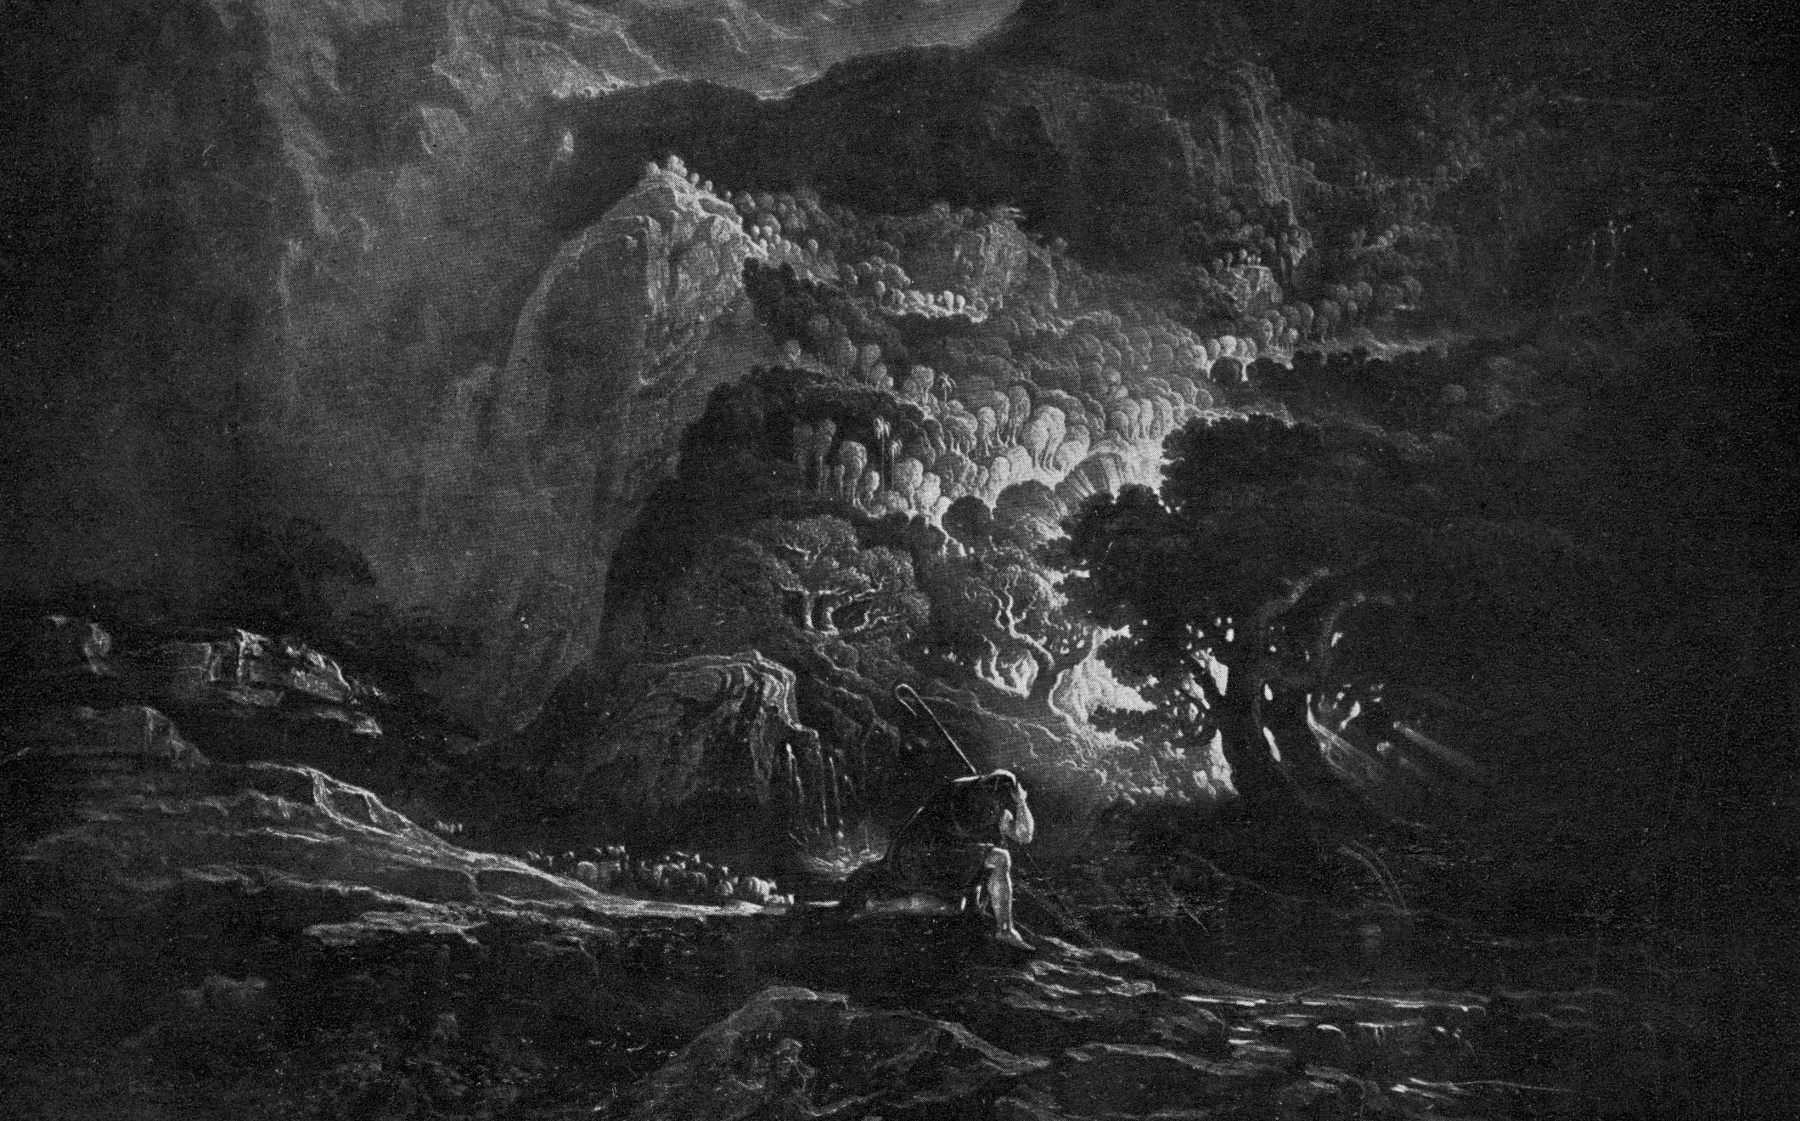
\includegraphics[width=1.3\linewidth]{burning_bush.jpg}}
    \caption{\hspace*{4cm}Rubus Ardēns}
\end{figure}

Moysēs autem pāscēbat ovēs Iethrō socerī suī sacerdōtis Madian:
\marginpar{mināre: cōgere animālia}cumque mināsset gregem ad interiōra dēsertī,
venit ad montem Deī Horeb.
\marginpar{rubus, -ī (m): quaedam planta spinosa}
Appāruitque eī Dominus in flammā ignis dē mediō rubī:
\marginpar{ārdēre: igne flagrāre}\marginpar{combūrere: igne cōnsūmere}et vidēbat quod rubus ārdēret, et nōn combūrerētur.
Dīxit ergō Moysēs : ``Vādam, et vidēbō vīsiōnem hanc magnam, quārē nōn combūrātur rubus.''

Cernēns autem Dominus quod pergeret ad videndum,
vocāvit eum dē mediō rubī, et ait: ``Moysēs, Moysēs.''

Quī respondit: ``Adsum.''

\marginpar{calceāmentum, -ī: quod pedī induitur}At ille: ``Nē appropiēs,'' inquit, ``hūc: solve calceāmentum dē pedibus tuīs: locus enim,
in quō stās, terra sāncta est.'' 

Et ait: ``Ego sum Deus patris tuī, Deus Abraham, Deus Isaac et Deus Iācōb.''

Abscondit Moysēs faciem suam: nōn\linebreak enim audēbat aspicere contrā Deum.

\marginpar{afflīctiō, -ōnis (f): rēs quae valde displicet, vexat, nocet}Cui ait Dominus: ``Vīdī afflīctiōnem populī meī in Ægyptō,
\marginpar{{\bf duritia, -ae (f)} $<$ durus/a/um}et clāmōrem eius audīvī propter dūritiam eōrum quī præsunt operibus:
et sciēns dolōrem eius, dēscendī ut libērem eum dē manibus Ægyptiōrum,
\marginpar{spatiōsus/a/um: multum spatiī habēns}et ēdūcam dē terrā illā in terram bonam, et spatiōsam,
\marginpar{lac, lactis (n): quod infantēs bibunt}in terram quæ fluit lacte et melle,
ad loca Chananæī et Hethæī, et Amorrhæī, et Pherezæī, et Hevæī, et Iebusæī.
Clāmor ergō fīliōrum Isrāēl venit ad mē: vīdīque afflīctiōnem eōrum,
qua ab Ægyptiīs opprimuntur.
Sed vēnī, et mittam tē ad Pharaōnem,
ut ēducās populum meum, fīliōs Isrāēl, dē Ægyptō.''

Dīxitque Moysēs ad Deum: ``Quis sum ego ut vādam ad Pharaōnem,
et ēdūcam fīliōs Isrāēl dē Ægyptō?''

Quī dīxit eī: ``Ego erō tēcum: et hoc habēbis signum,
quod mīserim tē: cum ēdūxerīs populum meum dē Ægyptō,
immolābis Deō super montem istum.''

Ait Moysēs ad Deum: ``Ecce ego vādam ad fīliōs Isrāēl,
et dīcam eīs: Deus patrum vestrōrum mīsit mē ad vōs.
Sī dīxerint mihi: `Quod est nōmen eius?' quid dīcam eīs?''

Dīxit Deus ad Moysēn: ``EGO SUM QUĪ SUM.'' Ait: ``Sīc dīcēs fīliīs Isrāēl: `QUĪ EST mīsit mē ad vōs.' ''

Dīxitque iterum Deus ad Moysēn: ``Hæc dīcēs fīliīs Isrāēl:
Dominus Deus patrum vestrōrum, Deus Abraham, Deus Isaac et Deus Iācōb,
\marginpar{in æternum: semper} mīsit mē ad vōs: hoc nōmen mihi est in æternum,
\marginpar{memoriāle, -is (n): id quod memorandum est}et hoc memoriāle meum in generātiōnem et generātiōnem.''

``Vāde, et congregā seniōrēs Isrāēl,
et dīcēs ad eōs: Dominus Deus patrum vestrōrum appāruit mihi,
Deus Abraham, Deus Isaac et Deus Iācōb,
\marginpar{vīsitāns vīsītāvī: vīsitāvī (rhētoricē paene idem iterum dicit)}dīcēns: Vīsitāns vīsitāvī vōs: et vīdī omnia quæ accidērunt vōbīs in Ægyptō.
Et dīxī ut ēdūcam vōs dē afflīctiōne Ægyptī in terram Chananæī,
et Hethæī, et Amorrhæī, et Pherezæī, et Hevæī, et Iebusæī,
ad terram fluentem lacte et melle.''

``Et audient vōcem tuam: ingrediērisque tū,
et seniōrēs Isrāēl, ad rēgem Ægyptī, et dīcēs ad eum:
Dominus Deus Hebræōrum vocāvit nōs:
\marginpar{sōlitūdo, -inis $<$ solus/a/um: regio deserta; locus ubi nemo vel unus habitat}ībimus viam trium diērum in sōlitūdinem,
\marginpar{immolāre: sacrificium facere}ut immolēmus Dominō Deō nostrō.''

``Sed ego sciō quod nōn dīmittet vōs rēx Ægyptī
ut eātis nisi per manum validam.
Extendam enim manum meam, et percutiam Ægyptum
in cūnctīs mīrābilibus meīs, 
quæ factūrus sum in mediō eōrum:
post hæc dīmittet vōs.
Dabōque grātiam populō huic cōram Ægyptiīs:
\marginpar{vacuī: id est, sine rēbus}et cum ēgrediēminī, nōn exībitis vacuī:
\marginpar{vīcīnus/a: qui prope habitat}sed postulābit mulier ā vīcīnā suā
et ab hospitā suā, vāsa argentea et aurea, ac vestēs:
\marginpar{spoliāre: capere rēs aliōrum hominum}pōnētisque eās super fīliōs et fīliās vestrās, et spoliābitis Ægyptum.''

\section{Quaestiō Augustinī}

``Clāmāvit illum Dominus dē rubō.''

\marginpar{in angelō: in formā angelī (?)}Dominus in angelō? an Dominus, angelus ille quī dictus est: 
``Magnī cōnsiliī angelus,'' (Isa 9:6) et intellegitur Chrīstus? 
Suprā enim dīxit: ``Appāruit illī angelus Dominī in flammā ignis dē rubō.''

\section{Quaestiō Augustinī Altera}

``Ēdūcere illōs dē terrā illa in terram bonam et
multam, in terram fluentem lac et mel.'' 

\marginpar{spīritāliter (adv.): secundum spiritum}Utrum terram fluentem lac et mel spīritāliter accipere
\marginpar{proprietas (verborum): conjunctio illorum arta et apta cum rebus ipsis, quas significant}dēbēmus? quia secundum proprietātem nōn hoc erat
illa quae data est populō Isrāēl? 
an locūtiōnis est, quā id ad laudem ūbertātis et suāvitātis referātur?

\chapter{CAPITULUM QUARTUM}

\begin{figure}[h]
    \hspace*{0.5cm}
    \setlength{\fboxsep}{0pt}
    \fbox{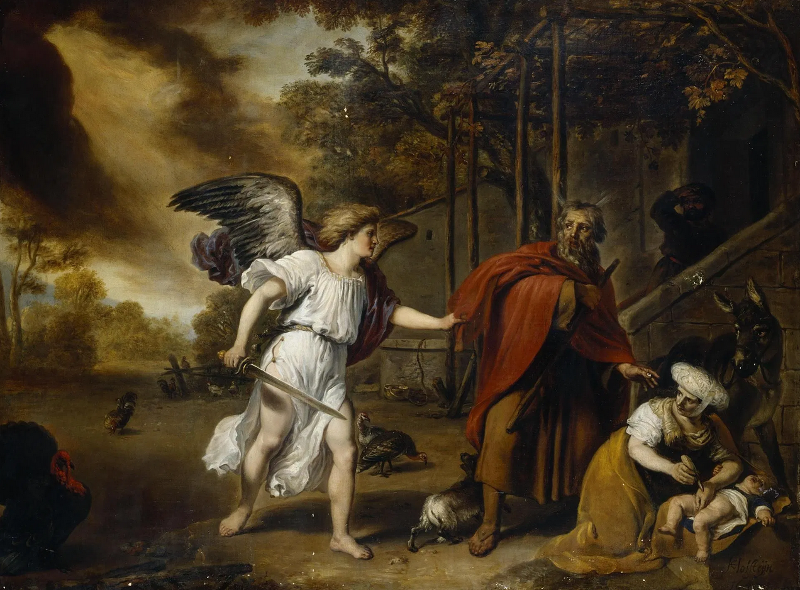
\includegraphics[width=1.3\linewidth]{inn.png}}
    \caption{\hspace*{4cm}Sephora in Deversōriō}
\end{figure}

Respondēns Moysēs ait: ``Nōn crēdent mihi, neque audient vōcem meam, sed dīcent:
Nōn appāruit tibi Dominus.''

Dīxit ergō ad eum: ``Quid est quod tenēs in manū tuā?''

Respondit: ``Virga.''

\marginpar{prōiicere: procul iacere; abiicere} Dīxitque Dominus: ``Prōiice eam in terram.''

\marginpar{coluber, -brī (m): serpens}Prōiēcit, et versa est in colubrum, ita ut fugeret Moysēs. 

Dīxitque Dominus: ``Extende manum tuam, et apprehende caudam eius.''

Extendit, et tenuit, versaque est in virgam.
``Ut crēdant,'' inquit, ``quod appāruerit tibi Dominus Deus patrum suōrum,
Deus Abraham, Deus Isaac et Deus Iācōb.''

Dīxitque Dominus rūrsum: ``Mitte manum tuam in sinum tuum.''

\marginpar{{\bf leprōsus/a/um $<$ leprae, -ārum (f)}: morbus qui cutem (exterior pars hominis) deformat}
\marginpar{īnstar + gen: sicut}Quam cum mīsisset in sinum, prōtulit leprōsam īnstar nivis.
``Retrahe,'' ait, ``manum tuam in sinum tuum.''

Retrāxit, et prōtulit iterum,
et erat similis carnī reliquæ.
``Sī nōn crēdiderint,'' inquit, ``tibi, neque audierint
sermōnem signī priōris, crēdent verbō signī sequentis. 
Quod sī nec duōbus quidem hīs signīs crēdiderint,
neque audierint vōcem tuam: sūme aquam flūminis,
\marginpar{āridus/a/um: sine aquā}et effunde eam super āridam, et quidquid hauserīs dē fluviō,
vertētur in sanguinem.''

\marginpar{nūdiustertius: ante duōs diēs}
Ait Moysēs: ``Obsecrō, Domine, nōn sum ēloquēns ab heri et
\marginpar{{\bf ex quō} (tempore)}nūdiustertius: et ex quō locūtus es ad servum tuum,
impedītiōris et tardiōris linguæ sum.''

Dīxit Dominus ad eum: ``Quis fēcit os hominis?
\marginpar{fabricatus/a/um: confectus}
\marginpar{mūtus/a/um: loquī non potest}
\marginpar{surdus/a/um: audīre non potest}
aut quis fabricātus est mūtum et surdum,
\marginpar{caecus/a/um: vidēre non potest}videntem et cæcum? nōnne ego?
Perge, igitur, et ego erō in ōre tuō:
docēbōque tē quid loquāris.''

\marginpar{obsecrāre: orāre, precārī}At ille: ``Obsecrō, inquit, Domine,
mitte quem missūrus es.''

Īrātus Dominus in Moysēn, ait: ``Aarōn frāter tuus Lēvītēs,
sciō quod ēloquēns sit: ecce ipse ēgreditur in occursum tuum,
vidēnsque tē lætābitur corde.
Loquere ad eum, et pōne verba mea in ōre eius:
et ego erō in ōre tuō, et in ōre illīus,
et ostendam vōbīs quid agere dēbeātis.
Ipse loquētur prō tē ad populum,
et erit os tuum:
tū autem eris eī in hīs quæ ad Deum pertinent.
Virgam quoque hanc sūme in manū tuā,
in quā factūrus es signa.

\marginpar{socer, socerī (m): pater uxōris}Abiit Moysēs, et reversus est ad Iethrō socerum suum,
dīxitque eī: ``Vādam et revertar ad frātrēs meōs in Ægyptum,
ut videam sī adhūc vīvant.''

Cui ait Iethrō: ``Vāde in pāce.''

Dīxit ergō Dominus ad Moysēn in Madiān: ``Vāde, et revertere in Ægyptum,
mortuī sunt enim omnēs quī quærēbant animam tuam.''

\begin{figure}[hbp]
        \centering
        \setlength{\fboxsep}{0pt}
        \fbox{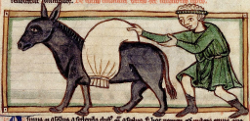
\includegraphics{asinus}}
        \caption{asinus, -ī (m)}
\end{figure}
Tulit ergō Moysēs uxōrem suam, et fīliōs suōs,
et imposuit eōs super asinum: reversusque est in Ægyptum,
portāns virgam Deī in manū suā. Dīxitque eī Dominus revertentī
in Ægyptum: ``Vidē ut omnia ostenta quæ posuī in manū tuā
\marginpar{indūrāre: durum facere}faciās cōram Pharaōne: ego indūrābō cor eius,
et nōn dīmittet populum. Dīcēsque ad eum: Hæc
\marginpar{prīmōgenitus: natū maior}dīcit Dominus: Fīlius meus prīmōgenitus Isrāēl.
Dīxī tibi: Dīmitte fīlium meum ut serviat mihi;
et nōluistī dīmittere eum:
ecce ego interficiam fīlium tuum prīmōgenitum.''

\marginpar{dīversōrium, -ī (n): aedificium in quō hominēs in itinere possunt dormīre}\marginpar{petra, -ae (f): lapis}Cumque esset in itinere, in dīversōriō
occurrit eī Dominus, et volēbat occīdere eum. 
\marginpar{idcircō: proptereā, ideō}Tulit idcircō Sephora acūtissimam petram,
\marginpar{praepūtium, -ī (n): illa pars puerī quae circumcīditur}et circumcīdit præpūtium fīliī suī, tetigitque pedēs ejus,
\marginpar{spōnsus/a: quī mox alicui maritus vel uxor erit}et ait: ``Spōnsus sanguinum tū mihi es.''
Et dīmīsit eum postquam dīxerat: ``Spōnsus sanguinum ob circumcīsiōnem.''

Dīxit autem Dominus ad Aarōn: ``Vāde in occursum Moȳsī
in dēsertum.'' 

Quī perrēxit obviam eī in montem Deī, et ōsculātus est eum.
Nārrāvitque Moysēs Aarōn omnia verba Dominī quibus miserat eum,
et signa quæ mandāverat. Vēnēruntque simul, et congregāvērunt
cūnctōs seniōrēs fīliōrum Isrāēl.
Locūtusque est Aarōn omnia verba quæ dīxerat Dominus ad Moysēn: et
fēcit signa cōram populō, et crēdidit populus.
Audiēruntque quod vīsitāsset Dominus fīliōs Isrāēl,
\marginpar{prōnus/a/um: iacēns in pectore}et respexisset afflīctiōnem illōrum: et prōnī adōrāvērunt.

\section{Quaestiō Augustinī}

Quemadmodum possit intellegī īrāscēns\linebreak
Deus, quia nōn sīcut homō per irratiōnābilem perturbātiōnem, per omnia
tenendum est, ubi tāle aliquid Scrīptūra dīcit, nē dē hōc eadem saepe
dīcenda sint. Sed meritō quaeritur cūr hīc īrātus dē frātre Moyse
dīxerit, quod ipse illī loquerētur ad populum: vidētur enim tamquam
\marginpar{diffīdere: nōn fīdere}diffīdentī nōn dedisse plēnissimam facultātem, quam datūrus erat; et per 
duōs agī voluisse, quod et per ūnum posset, sī crēdidisset.

Vērumtamen
eadem verba omnia dīligentius cōnsīderāta, nōn significant īrātum
\marginpar{vindicta, -ae (f): ultio vel animadversio pro delicto;
vindicatio}Dominum prō vindictā dedisse Aarōn. Sīc enim dīcit: ``Nōnne ecce Aarōn
frāter tuus Lēvītēs? sciō quia loquēns loquētur ipse.''

Quibus verbīs
ostenditur Deus increpāsse potius eum, quī timēret īre quod ipse esset
minus idōneus, cum habēret frātrem per quem posset ad populum loquī quod
\marginpar{gracilis, -is (adj): tenuis, exilis}vellet; quoniam erat ipse gracilis vōcis, et linguae tardiōris: quamquam
dē Deō tōtum spērāre dēbēret. Deinde eadem ipsa quae paulō ante
prōmīserat, et posteāquam īrātus est, dīcit. Dīxerat enim: ``Aperiam os
tuum, et īnstruam tē''; nunc autem dīcit: ``Aperiam os tuum et os eius, et
īnstruam vōs quae faciātis''; sed quoniam addidit: ``Et loquētur ipse tibi
ad populum,'' vidētur ōris apertiō praestita, propter quod dīcit Moysēs
linguae sē esse tardiōris. 

Dē vōcis autem gracilitāte nihil eī praestāre
\marginpar{adiūtōrium, -ī (n): auxilium, quodqumque adiuvat}Dominus voluit, sed propter hoc adiūtōrium frātris adiūnxit, quī posset
eā utī vōce, quae pōpulō docendō sufficeret. Quod ergō ait: ``Et dabis
verba mea in os eius,'' ostendit quod ea loquenda esset datūrus: nam sī
\marginpar{tantummodo: solum, solummodo}tantummodo audienda, sīcut populō, in aurēs dīceret. Deinde quod paulō
post ait: ``Et loquētur ipse tibi ad populum, et ipse erit tuum os, et hic
subaudītur, ad populum.'' Et cum dīcit: ``Tibi loquētur ad populum''; satis
indicat in Moysēn prīncipātum, in Aarōn ministerium. Deinde quod ait: ``Tū
\marginpar{fortassis = fortasse}autem illī eris quae ad Deum,'' magnum
hīc fortassis perscrūtandum 
\marginpar{sacrāmentum, -ī: mysterium, signum sensibile rei sacrae
latentis}est sacrāmentum, cuius figūram gerat, velutī medius Moysēs inter Deum et
Aarōn, et medius Aarōn inter Moysēn et populum. 

\section{Quaestio Augustini Altera}

\marginpar{obviāre: obviam īre}In eō quod scrīptum est: Et factum est, in viā ad refectiōnem obviāvit
\marginpar{calculus: parvus lapis}eī angelus, et quaerēbat eum occīdere: et assūmptō Sepphora calculō,
\marginpar{praepūtium, -ī (n): illa pars puerī quae circumcīditur}circumcīdit praepūtium fīliī suī; et prōcidit ad pedēs eius, et dīxit:
``Stetit sanguis circumcīsiōnis īnfantis meī. Et recessit ab eō;'' propter
quod dīxit: ``Dēsiit sanguis circumcīsiōnis;'' 

Prīmum quaeritur, quem
volēbat angelus occīdere, utrum Moysen, quia dictum est, ``occurrit eī
angelus, et quaerēbat eum occīdere.'' Nam cui putābitur occurrisse, nisi
\marginpar{comitātus, -ūs (m): comitum multitudo}illī quī ūniversō suōrum comitātuī praefuit, et ā quō caeterī
dūcēbantur? An puerum quaerēbat occīdere, cui māter circumcīdendō
\marginpar{subvenīre: opem ferre, auxiliari, succurrere}subvenit; ut ob hoc intellegātur occīdere voluisse īnfantem, quia nōn
\marginpar{sancīre: aliquid ritu sacro, seu religioso decernere,
constituere}erat circumcīsus, atque ita sancīre praeceptum circumcīsiōnis,
sevēritāte vindictae?

Quod sī ita est, incertum est prius dē quō
\marginpar{id est, ut ita dicam, quis est ``eum''? Quis est ``eī''?}dīxerit, ``quaerēbat eum occīdere;'' quia ignōrātur quem, nisi ex
cōnsequentibus reperiātur: mīrā sānē locūtiōne et inūsitātā, ut prius
dīceret, ``occurrit eī,'' et quaerēbat eum occīdere, dē quō nihil anteā
dīxerat.

Sed tālis est in Psalmō: ``Fundāmenta eius in montibus sānctīs;
dīligit Dominus portās Sīōn.'' Inde enim Psalmus incipit, nec aliquid
dē illō vel dē illā dīxerat, cuius fundāmenta intellegī voluit, dīcēns:
Fundāmenta eius in montibus sānctīs. Sed quia sequitur, ``dīligit Dominus
portās Sīōn,'' ergō fundāmenta vel Dominī vel Sīōn, et ad faciliōrem
sēnsum magis Sīōn, ut fundāmenta cīvitātis accipiantur. Sed quia in hōc
prōnōmine, quod est, ``eius,'' genus ambiguum est (omnis enim generis est
hoc prōnōmen, id est et masculīnī, et fēminīnī, et neutrī), in graecō
autem in fēminīnō genere ``autes'' dīcātur, masculīnō et neutrō
``autou'', et habet cōdex
graecus ``autou'', cōgit intellegere nōn fundāmenta Sīōn, sed fundāmenta Dominī,
id est, quae cōnstituit Dominus, dē quō dictum est: ``Aedificāns Ierusālem
Dominus.'' Nec Sīōn tamen, nec Dominum anteā nōmināverat, cum dīceret:
``Fundāmenta eius in montibus sānctīs.'' 

Sīc et hīc nōndum nōminātō īnfante
dictum est, ``occurrit eī, et quaerēbat eum occīdere;'' ut dē quō dīxerit,
in cōnsequentibus agnōscāmus.  Quamquam etsī dē Moyse accipere quisquam
\marginpar{magnopere: valde, vehementer}voluerit, nōn est magnopere resistendum.

Illud potius quod sequitur, sī
fierī potest, intellegātur, quid sibi velit ideō recessisse angelum ab
interfectiōne cuiuslibet eōrum, quia dīxit mulier: ``Stetit sanguis
circumcīsiōnis īnfantis.'' Nōn enim ait: Recessit ab eō, propter quod
circumcīdit īnfantem: sed quia stetit sanguis circumcīsiōnis; nōn quia
cucurrit, sed quia stetit: magnō, nisi fallor, sacrāmentō. 

\chapter{CAPITULUM QUINTUM}

Post hæc ingressī sunt Moysēs et Aarōn,
et dīxērunt Pharaōnī: ``Hæc dīcit Dominus Deus Isrāēl:
Dīmitte populum meum ut sacrificet mihi in dēsertō.''

At ille respondit: ``Quis est Dominus,
ut audiam vōcem ejus, et dīmittam Isrāēl?
Nesciō Dominum, et Isrāēl nōn dīmittam.''

Dīxēruntque: ``Deus Hebræōrum vocāvit nōs,
ut eāmus viam trium diērum in sōlitūdinem,
et sacrificēmus Dominō Deō nostrō:
\marginpar{pestis, -is (f): aliquid malum - morbus, calamitas, cēt.}nē forte accidat nōbīs pestis aut gladius.''

\marginpar{sollicitāre: invitāre, allicere}Ait ad eōs rēx Ægyptī: ``Quārē Moysēs et Aarōn sollicitātis populum ab operibus suīs? Īte ad onera vestra.''

Dīxitque Pharaō: ``Multus est populus terræ:
\marginpar{succrēscere (sub + crēscere): ab īmō crēscere}vidētis quod turba succrēverit:
quantō magis sī dederītis eīs requiem ab operibus?''

Præcēpit ergō in diē illō præfectīs operum
et exāctōribus populī, dīcēns: 
``Nēquāquam ultrā dabitis paleās populō ad cōnficiendōs laterēs,
sīcut prius: sed ipsī vadant, et colligant stipulās.
Et mēnsūram laterum, quam prius faciēbant,
impōnētis super eōs, nec minuētis quidquam:
\marginpar{idcircō: proptereā, ideō}vacant enim, et idcircō vōciferantur, dīcentēs:
Eāmus, et sacrificēmus Deō nostrō.
Opprimantur operibus, et expleant ea:
ut nōn acquiēscant verbīs mendācibus.''

\marginpar{praefectus, -ī (m): qui alicui rei vel negotio praepositus est}Igitur ēgressī præfectī operum et exāctōrēs ad populum,
\marginpar{exāctōr, -ī: qui facit ut opera perficiantur}
dīxērunt: Sīc dīcit Pharaō: ``Nōn dō vōbīs paleās: īte,
et colligite sīcubi invenīre poteritis,
nec minuētur quidquam dē opere vestrō.''

\kimg{palea}{paleam colligentes}
Dispersusque est populus per omnem terram Ægyptī ad colligendās paleās.
Præfectī quoque operum
\marginpar{quotīdiē: cotīdiē}īnstābant, dīcentēs: ``Complētē opus vestrum quotīdiē,
ut prius facere solēbātis quandō dabantur vōbīs paleæ.''

\begin{figure}[H]
    \begin{minipage}[]{0.5\linewidth}
        \centering
        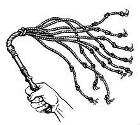
\includegraphics{flagellum}
        \caption{flagellum, -ī (n)}
    \end{minipage}%
    \begin{minipage}[]{0.5\linewidth}
        \centering
        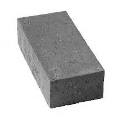
\includegraphics{later}
        \caption{later, lateris (m)}
    \end{minipage}
\end{figure}
\marginpar{flagellāre: flagellīs pulsāre}Flagellātīque sunt quī præerant operibus fīliōrum Isrāēl,
ab exāctōribus Pharaōnis, dīcentibus: ``Quārē nōn implētis
mēnsūram laterum sīcut prius, nec heri, nec hodiē?''

Vēnēruntque præpositī fīliōrum
\marginpar{vōciferārī: vehementer exclamāre}Isrāēl, et vōciferātī sunt ad Pharaōnem
dīcentēs: \linebreak``Cūr ita agis contrā servōs tuōs?
Paleæ nōn dantur nōbīs, et laterēs similiter
\marginpar{ēn: ecce}imperantur: ēn famulī tuī flagellīs cædimur,
et iniūstē agitur contrā populum tuum.''

\marginpar{idcircō: proptereā, ideō}Quī ait: ``Vacātis ōtiō,
et idcircō dīcitis: 
Eāmus, et sacrificēmus Dominō. 
\marginpar{operārī: laborāre}Īte ergō, et operāminī: paleæ
\marginpar{cōnsuētus numerus: numerus quod semper antea erat}nōn dabuntur vōbīs, et reddētis cōnsuētum numerum laterum.''

\marginpar{eō quod: quia}Vidēbantque sē præpositī fīliōrum Isrāēl
in malō, eō quod dīcerētur eīs: ``Nōn minuētur quidquam
dē lateribus per singulōs diēs.''

Occurrēruntque Moȳsī et Aarōn, quī stābant ex adversō,
ēgredientibus ā Pharaōne: et dīxērunt
ad eōs: ``Videat Dominus et jūdicet, quoniam
\marginpar{fœtēre: male olēre (rēs olēns afficit nāsum)}fœtēre fēcistis odōrem nostrum cōram Pharaōne
\marginpar{præbēre: dāre}et servīs eius, et præbuistis eī
gladium, ut occīderet nōs.'' 

Reversusque est Moysēs ad Dominum, et ait: ``Domine, cūr
\marginpar{ex eō: ex eō (tempore)}afflīxistī populum istum? Quārē mīsistī mē? Ex eō
enim quō ingressus sum ad Pharaōnem ut
loquerer in nōmine tuō, afflīxit populum
tuum: et nōn līberāstī eōs.''

\section{Quaestiō Augustīnī}

Quaeritur quōmodo populō dīcātur, quod mandāvit Deus ēiectūrum sē eōs dē
Aegyptō in terram Chanaan; Pharaōnī autem dīcātur, quod trium diērum
iter exīre vellent in dēsertum immolāre Deō suō ex mandātō eius.

Sed intellegendum est,\marginpar{quamvīs: etsī} quamvīs Deus scīret quid esset factūrus, quoniam
praesciēbat nōn cōnsēnsūrum Pharaōnem ad populum dīmittendum, illud
prīmō dictum esse, quod etiam \marginpar{prīmitus (adv): primum, primo}prīmitus fieret, sī ille dīmitteret. Ut
enim sīc fierent omnia quemadmodum cōnsequēns Scrīptūra testātur,
Pharaōnis \marginpar{contumācia, -ae (f): superbia}contumācia meruit et suōrum. Neque enim mendāciter Deus iubet
quod scit nōn factūrum cui iubētur, ut iūstum iūdicium cōnsequātur. 

\section{Quaestiō Augustīnī Altera}

Verba quae dīcit Moysēs ad Dominum: ``Quārē afflīxistī populum hunc? et
\marginpar{utquid: quamobrem}utquid mē mīsistī? Ex quō enim intrāvī ad Pharaōnem loquī in tuō nōmine,
in hunc populum; et nōn līberāstī populum tuum.'' Nōn contumāciae verba
sunt vel indignātiōnis, sed inquīsītiōnis et ōrātiōnis: quod ex hīs
appāret, quae illī Dominus respondit. Nōn enim arguit īnfidēlitātem
eius, sed quid sit factūrus aperuit.

\chapter{CAPITULUM SEXTUM}

Dīxitque Dominus ad Moysēn: ``Nunc vidēbis quæ factūrus
sim Pharaōnī: per manum enim fortem dīmittet
\marginpar{rōbustus/a/um: durus, rigidus, valens}eōs, et in manū rōbustā ēiiciet illōs
dē terrā suā.''

Locūtusque est Dominus ad Moysēn dīcēns: ``Ego Dominus
quī appāruī Abraham, Isaac et Iācōb
in Deō omnipotente: et nōmen meum Adonaī
\marginpar{pangō, pangere, pepigisse, pactum: constituere, definite statuere}\marginpar{foedus, foederis (n): res inter duōbus hominēs vel civitatēs constituta} nōn indicāvī eīs. Pepigīque fœdus cum eīs, ut
darem eīs terram Chanaan, terram peregrīnātiōnis
eōrum, in quā fuērunt advenæ. 
Ego audīvī gemitum fīliōrum Isrāēl, quō
Ægyptiī oppressērunt eōs: et recordātus
sum pactī meī. Ideō dīc fīliīs Isrāēl: Ego Dominus
\marginpar{ergastulum, -ī: carcer rusticus}quī ēdūcam vōs dē ergastulō Ægyptiōrum, et
ēruam dē servitūte, ac redimam in brāchiō
excelsō et jūdiciīs magnīs. Et assūmam vōs mihi
in populum, et erō vester Deus: et sciētis quod ego
sum Dominus Deus vester quī ēdūxerim vōs dē
ergastulō Ægyptiōrum, et indūxerim in terram, super quam
levāvī manum meam ut darem eam Abraham, Isaac
et Iācōb: dabōque illam vōbīs possidendam. 
Ego Dominus.''

Nārrāvit ergō Moysēs omnia fīliīs Isrāēl: quī nōn
\marginpar{acquiescere: assentiri, fidem habere}acquiēvērunt eī
propter angustiam spīritūs, et opus dūrissimum. Locūtusque est
Dominus ad Moysen, dīcēns: ``Ingredere, et loquere ad Pharaōnem rēgem
Ægyptī, ut dīmittat fīliōs Isrāēl dē terrā suā.''

Respondit Moysēs cōram Dominō: ``Ecce fīliī Isrāēl nōn audiunt mē: et
quōmodo audiet
\marginpar{``incircumcīsus labiīs'' fortasse sibi vult labia (id est,
facultas loquendi) non iam deo serviendo apta esse, sicut vir
incircumcisus non iam deo serviendo aptus est} Pharaō, præsertim cum incircumcīsus sim labiīs?'' 

Locūtusque est
Dominus ad Moysēn et Aarōn, et dēdit mandātum ad fīliōs Isrāēl, et ad
Pharaōnem rēgem Ægyptī ut ēdūcerent fīliōs Isrāēl dē terrā Ægyptī.

\chapter{CAPITULUM SEPTIMUM}

\kimg{mosph.jpg}{Moyses ante Pharaonem}

Dīxitque Dominus ad Moysēn: ``Ecce cōnstituī tē Deum Pharaōnis: et Aarōn
frāter tuus erit prophēta tuus. Tū loqueris eī omnia quæ mandō tibi:
et ille loquētur ad Pharaōnem, ut dīmittat fīliōs Isrāēl dē terrā suā. 
Sed ego indūrābō cor eius, et multiplicābō signa et ostenta mea in terrā
Ægyptī, et nōn audiet vōs: immittamque manum meam super Ægyptum, et
ēdūcam exercitum et populum meum fīliōs Isrāēl dē terrā Ægyptī per
iūdicia maxima. Et scient Ægyptiī quia ego sum Dominus quī extenderim
manum meam super Ægyptum, et ēdūxerim fīliōs Isrāēl dē mediō eōrum.''

Fēcit itaque Moysēs et Aarōn sīcut præcēperat Dominus: ita ēgerunt. 
Erat autem Moysēs octōgintā annōrum, et Aarōn octōgintā trium, quandō
locūtī sunt ad Pharaōnem.

Dīxitque Dominus ad Moysēn et Aarōn: ``Cum dīxerit vōbīs Pharaō,
Ostendite signa: dīcēs ad Aarōn: Tolle virgam tuam, et prōiice eam
\marginpar{coluber, -brī (m): serpens}cōram Pharaōne, ac vertētur in
colubrum.''

Ingressī itaque Moysēs et
Aarōn ad Pharaōnem, fēcērunt sīcut præcēperat Dominus: tulitque Aarōn
virgam cōram Pharaōne et servīs eius, quæ versa est in colubrum.
\marginpar{maleficus, -ī (m): magus, incantator}Vocāvit autem Pharaō sapientēs et maleficōs: et fēcērunt etiam ipsī per
incantātiōnēs ægyptiacās et arcāna quædam similiter. Prōiēcēruntque
\marginpar{dracō, -ōnis (m): serpens}singulī virgās suās, quæ versæ sunt in dracōnēs: sed dēvorāvit virga
Aarōn virgās eōrum. Indūrātumque est cor Pharaōnis, et nōn audīvit
eōs, sīcut præcēperat Dominus.

\marginpar{ingravāre: facere gravem}Dīxit autem Dominus ad Moysēn: ``Ingravātum est cor Pharaōnis: nōn vult
dīmittere populum. Vade ad eum māne, ecce ēgrediētur ad aquās: et
\marginpar{occursus, -ūs (m): obviam itio, actus occurendī}stābis in occursum eius super rīpam flūminis: et virgam quæ conversa
est in dracōnem, tollēs in manū tuā.  Dīcēsque ad eum: Dominus Deus
Hebræōrum mīsit mē ad tē, dīcēns: Dīmitte populum meum ut sacrificet
mihi in dēsertō: et usque ad præsēns audīre nōluistī. Hæc igitur
dīcit Dominus: In hōc sciēs quod sim Dominus: ecce percutiam virgā,
quæ in manū meā est, aquam flūminis, et vertētur in sanguinem. Piscēs
\marginpar{computrēscere: facere odorem malum propter res mortuas}quoque, quī sunt in fluviō, morientur, et computrēscent aquæ, et
afflīgentur Ægyptiī bibentēs aquam flūminis.''
\kimg{blood.jpg}{Moyses efficit ut flumen sit sanguineum}%

Dīxit quoque Dominus ad
Moysēn: ``Dīc ad Aarōn: Tolle virgam tuam, et extende manum tuam super
\marginpar{palus, palūdis (f): locus plenum aquae quae non fluit; aqua
stagnans}aquās Ægyptī, et super fluviōs eōrum, et rīvōs ac palūdēs, et omnēs
lacūs aquārum, ut vertantur in sanguinem: et sit cruor in omnī terrā
Ægyptī, tam in ligneīs vāsīs quam in saxeīs.''

Fēcēruntque Moysēs et
Aarōn sīcut præcēperat Dominus: et ēlevāns virgam percussit aquam
flūminis cōram Pharaōne et servīs eius: quæ versa est in sanguinem. 
Et piscēs, quī erant in flūmine, mortuī sunt: computruitque fluvius, et
nōn poterant Ægyptiī bibere aquam flūminis, et fuit sanguis in tōtā
terrā Ægyptī. 

Fēcēruntque similiter maleficī Ægyptiōrum
incantātiōnibus suīs: et indūrātum est cor Pharaōnis, nec audīvit eōs,
\mimg{fodit}{homō fodit}
sīcut præcēperat Dominus. Āvertitque sē, et ingressus est domum suam,
\marginpar{hāc vice: hāc occasione; nunc temporis}nec apposuit cor etiam hāc vice. Fōdērunt autem omnēs Ægyptiī per
circuitum flūminis aquam ut biberent: nōn enim poterant bibere dē aquā
flūminis. Implētīque sunt septem diēs, postquam percussit Dominus
fluvium.

\end{document}
